\documentclass[19pt,a4paper]{article}
\usepackage{xeCJK}
\usepackage{amsmath}
\setmainfont{STSong}
\usepackage{geometry}
\geometry{left=2.5cm,right=2.5cm,top=2.5cm,bottom=2.5cm}
\setlength{\parindent}{4em}
\usepackage{graphicx}
\usepackage{float}
\title{第三次实验报告}
\author{王诗俊2015201951\quad 廖钰蕾2015201953\quad  孟妍廷2015202009\quad  刘笑2015201925}
\date{2017年12月25日}

\begin{document}
\maketitle
\textbf{一\quad 阶段目标:}\\
\indent\ \  1.收集各类交通工具的图片作为训练集\\
\indent\ \  2.搭建神经网络识别各种交通工具\\
\indent\ \  3.使小车能在行驶时分析其拍到的交通工具的类别\\
\\
\\
\indent\textbf{二\quad 实现流程:}\\ 
\begin{figure}[H]
 \centering
 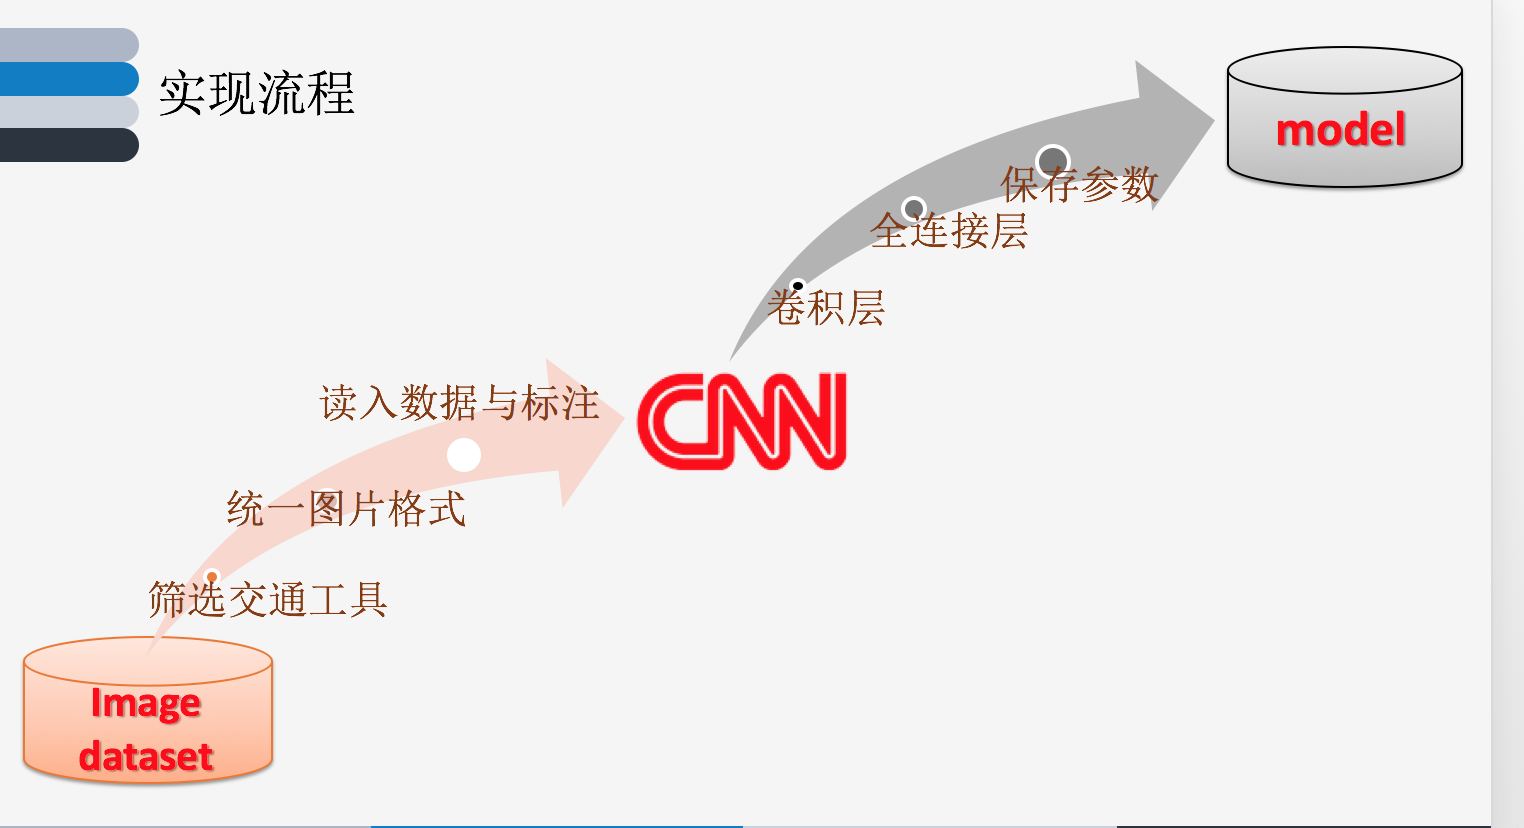
\includegraphics[scale=0.4]{流程1.png}
\end{figure}
\indent 首先,我们选择了一个已经标注好的大小为2G的图片集,从中筛选出拍摄对象是交通工具的图片并统一它们的的格式。把统一好的图片集作为训练集,搭建卷积神经网络,放入图片训练,得到model。
\begin{figure}[H]
 \centering
 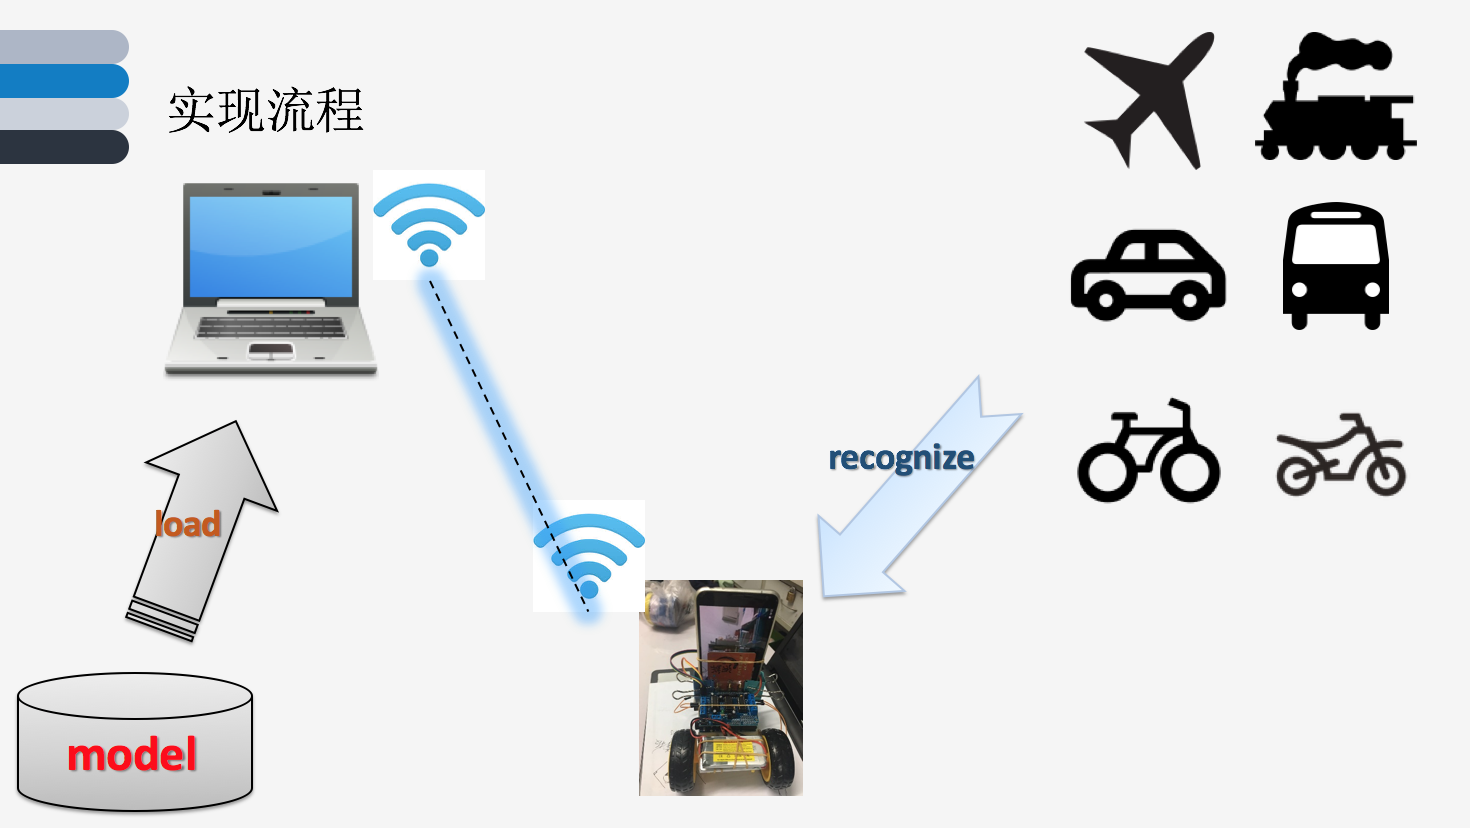
\includegraphics[scale=0.4]{流程2.png}
\end{figure}
\indent 接下来,把模型load进展示代码中,在小车上绑上手机摄像头,让小车在路上自由行驶并拍摄视频,把小车拍摄的视频中出现的交通工具截图出来,通过WiFi传回电脑,展示代码读入图片并利用model预测图片中的交通工具,最后把结果传给小车。
\\
\\
\indent\textbf{三\quad 代码逻辑:}\\
\indent ——数据预处理\\
\indent 1.下载PASCAL VOC2012图片集\\
\\
\indent 2.筛选\\
\indent \ \ 查看及分析下载的数据,将涉及到交通工具的图片类标注筛选出来\\
\\
\indent 3.处理\\
\indent \ \ 将所有的图片处理成100*100 大小的灰度图\\
\\
\indent 4.提取\\
\indent\ \ ImageSets中提取六类交通工具的测试集,并根据图片的特点,将各自的trainval修改标注,-1表示非,0~5表示图片对应的交通工具类 \\
\\
\indent 5.合并\\
\indent \ \ 为方便调用,将六类标注合成一个文档并筛重,得到最终的标注过的数据集\\
\\
\indent 6.形成矩阵并标注\\
\indent \ \ 调用程序,Xtrain是读入的图片处理成的矩阵,Ytrain是对应图片的标注\\
\\
\indent ——神经网络搭建\\
\indent 1.数据处理\\
\indent\ \ 数据集存成$(n \times100 \times100 \times 1)$大小的矩阵,随机分成训练集和测试集两部分\\
\indent 2.网络结构\\
\indent\ \ 采用一层卷积层+三层全连接层的网络结构,每一层后面采用reLU激活,卷积层后采用池化层降维,dropout层会抛弃一部分结点,防止过拟合,采用交叉熵作为损失函数\\
\indent 3.参数设置\\
\indent\ \ Filters:我们采用$100\times100$的图片,filters达到128\\
\indent\ \ Loss:多分类问题通常选用交叉熵作为损失函数\\
\indent\ \ Optimizer:选取adadelta,因为其学习率高,训练速度更快\\
\indent\ \ $Batch\_size:训练集大小为2620,batch\_size设为131$\\
\indent\ \ Epoch:取25,20次左右可充分收敛\\
\\
\\
\indent\textbf{四\quad 结果展示:}\\
\indent 1.识别正确率——90\%以上:\\
\indent\ \ 第一次训练时,卷积层的filters设为了64,在20\%的时候左右就收敛了;分析后发现图片尺寸较大,需要把filters设大一些,于是第二次训练改为了128,正确率得到了大大提高\\
\begin{figure}[H]
 \centering
 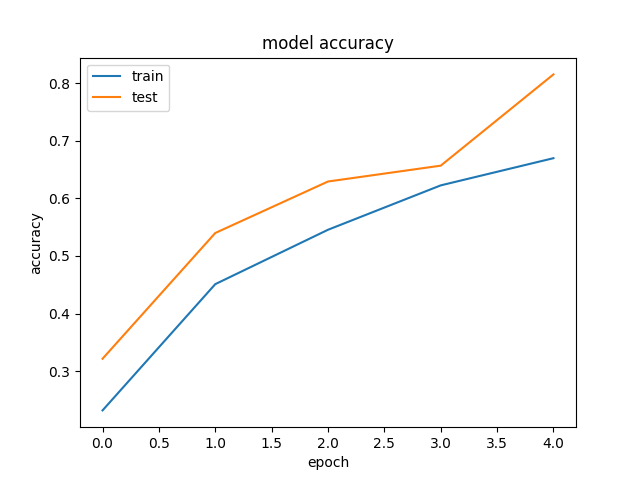
\includegraphics[scale=0.5]{acc.png}
\end{figure}
\indent 2.识别错误的情况
\begin{figure}[H]
 \centering
 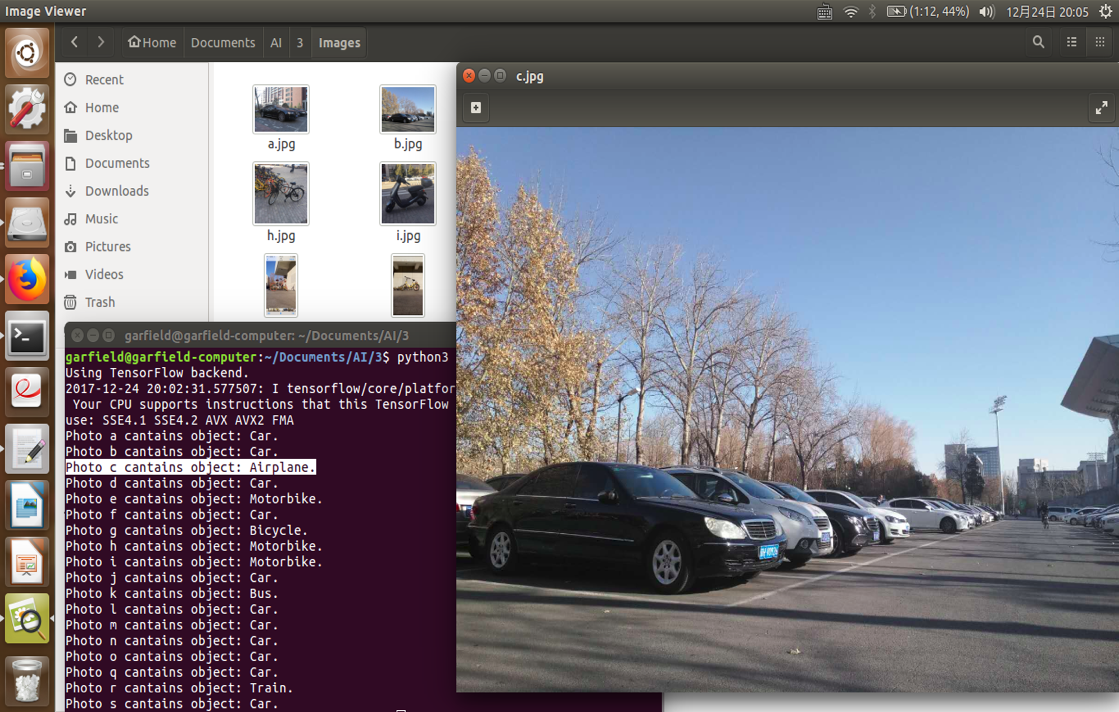
\includegraphics[scale=0.6]{wrong.png}
\end{figure}
\indent 图片中,车不是主角,留下来较大的天空和空地,有点类似于机场跑道。所以可能被model归类为飞机。\\
\indent 3.识别正确
\begin{figure}[H]
 \centering
 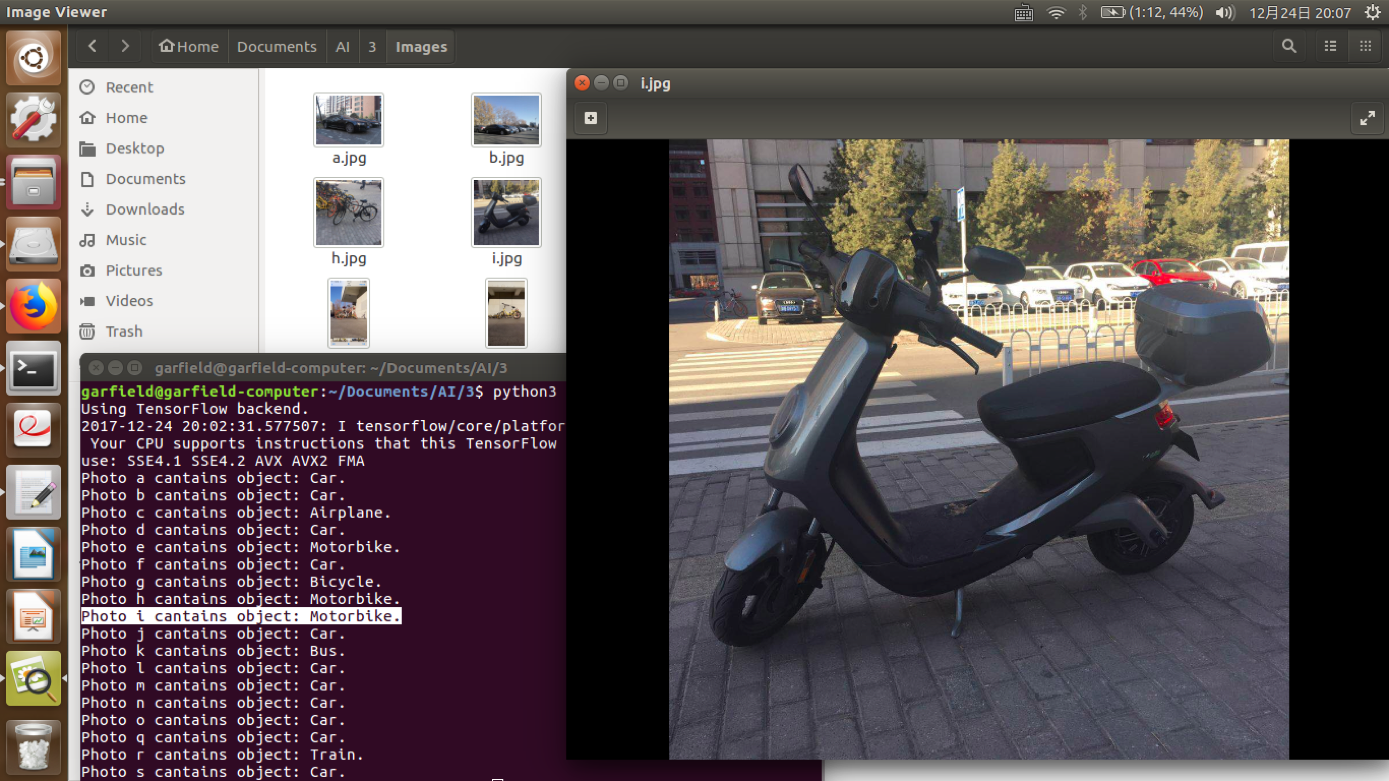
\includegraphics[scale=0.5]{right1.png}
\end{figure}
\begin{figure}[H]
 \centering
 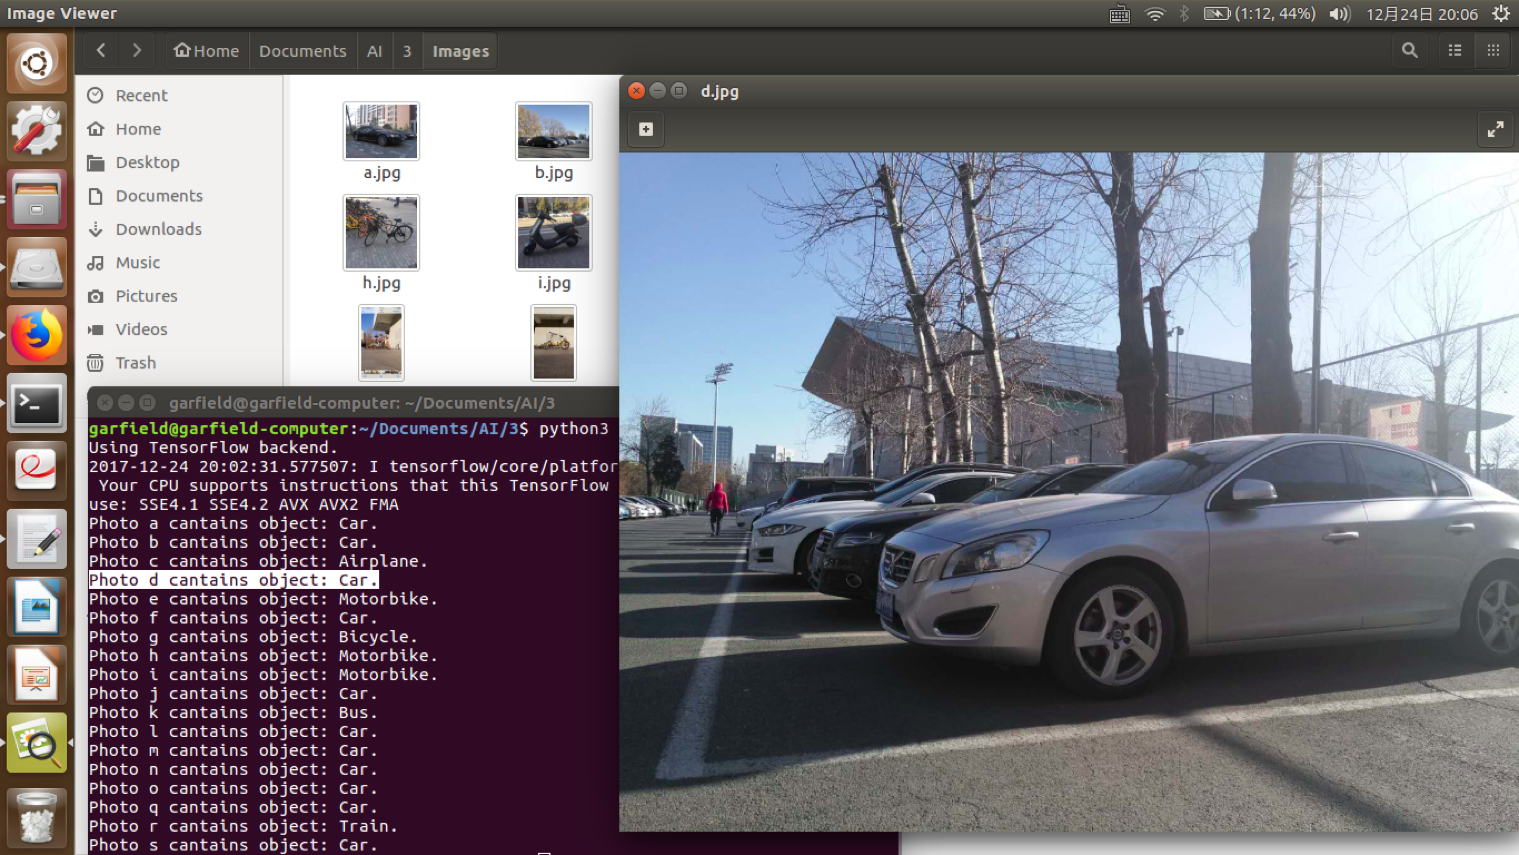
\includegraphics[scale=0.5]{right2.png}
\end{figure}
\begin{figure}[H]
 \centering
 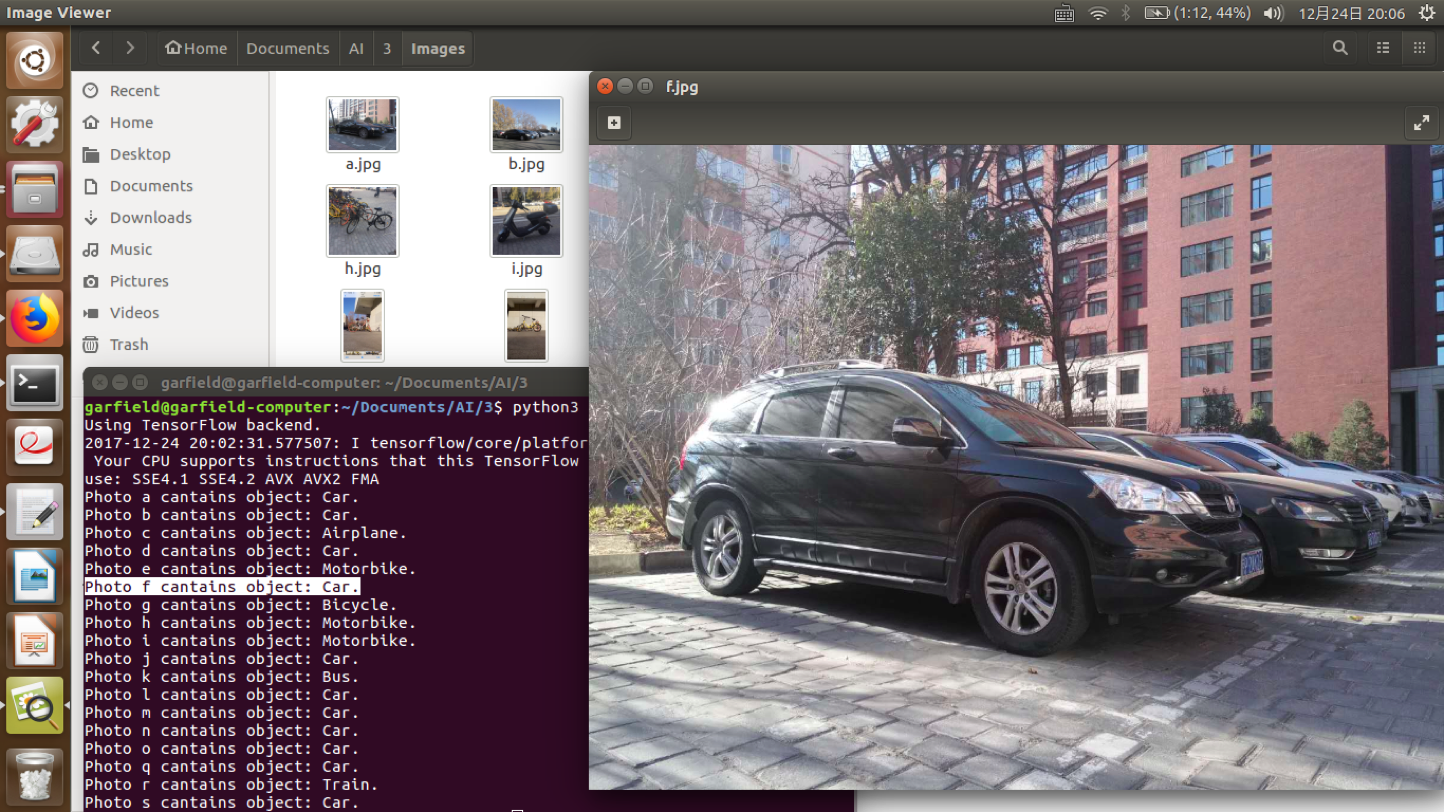
\includegraphics[scale=0.5]{right3.png}
\end{figure}
\begin{figure}[H]
 \centering
 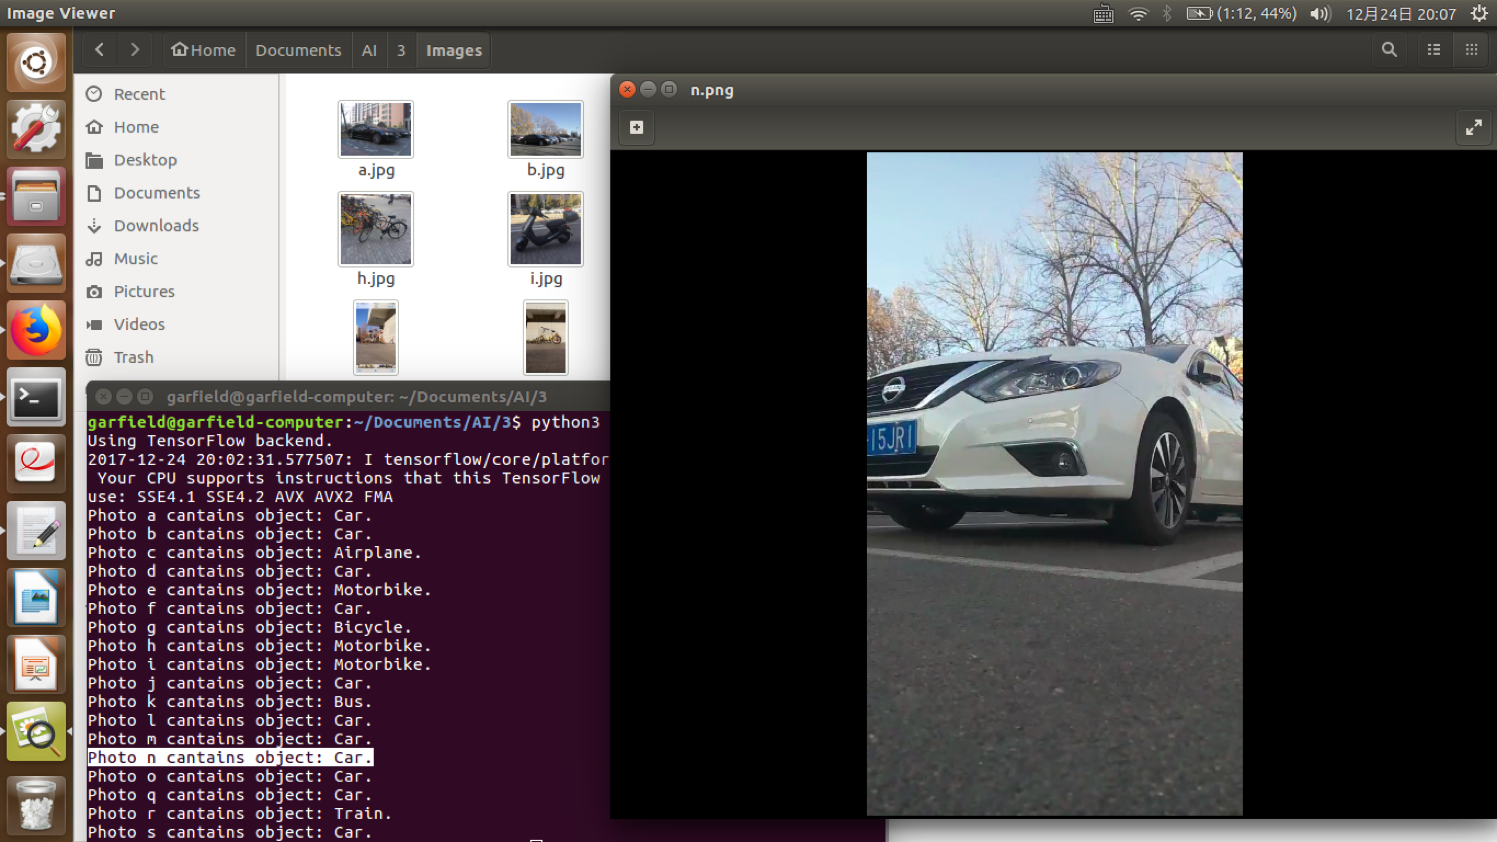
\includegraphics[scale=0.5]{right4.png}
\end{figure}
\indent 4.具体识别见视频\\
\\
\\
\indent\textbf{五\quad 分工:}\\
\begin{figure}[H]
 \centering
 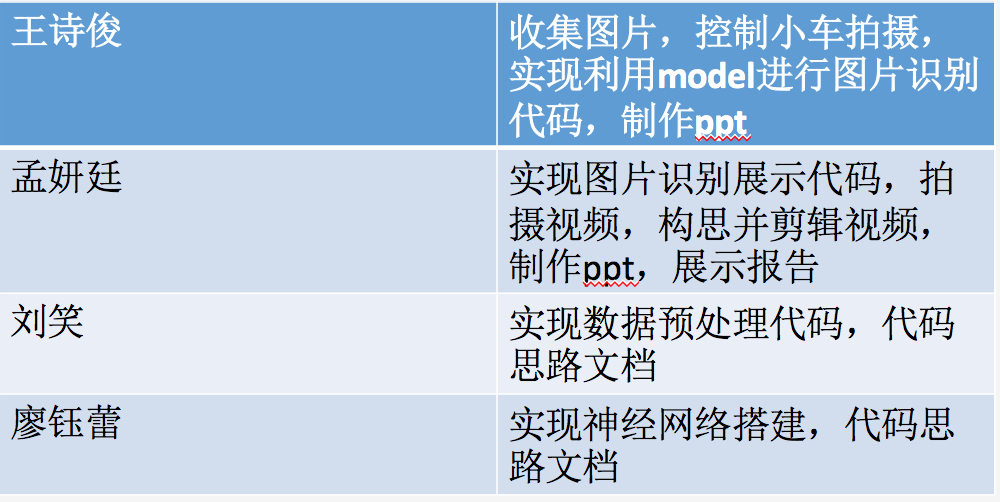
\includegraphics[scale=0.6]{分工.png}
\end{figure}


\end{document}